% ============================================================================
% DermAI: Quantifying Explanation Faithfulness and Localization
% in CNNs vs. Vision Transformers for Skin Lesion Classification
% CVPR-format submission
% ============================================================================

\documentclass[10pt,twocolumn,letterpaper]{article}

\usepackage{cvpr}
\usepackage{times}
\usepackage{epsfig}
\usepackage{graphicx}
\usepackage{amsmath}
\usepackage{amssymb}
\usepackage{booktabs}
\usepackage{multirow}
\usepackage{array}
\usepackage{color}
\usepackage{xcolor}
\usepackage{gensymb}
\usepackage{tabularx}
\usepackage{array}
\newcommand{\tablestrut}{\rule[-2pt]{0pt}{10pt}}

% Include other packages here, before hyperref.

% If you comment hyperref and then uncomment it, you should delete
% egpaper.aux before re-running latex.  (Or just hit 'q' on the first latex
% run, let it finish, and you should be clear).
\usepackage[pagebackref=true,breaklinks=true,letterpaper=true,colorlinks,bookmarks=false]{hyperref}

\cvprfinalcopy % *** Uncomment this line for the final submission

\def\cvprPaperID{****} % *** Enter the CVPR Paper ID here
\def\httilde{\mbox{\tt\raisebox{-.5ex}{\symbol{126}}}}

% Pages are numbered in submission mode, and unnumbered in camera-ready
\ifcvprfinal\pagestyle{empty}\fi
\raggedbottom

% ============================================================================
% MACROS
% ============================================================================

\newcommand{\rubrictitle}[1]{\textcolor{blue}{\textbf{[RUBRIC: #1]}}}
\newcommand{\todo}[1]{\textcolor{red}{\textbf{[TODO: #1]}}}
\providecommand{\etal}{\textit{et al.}}

\begin{document}

%%%%%%%%% TITLE

\title{Quantifying Explanation Faithfulness and Localization in CNNs vs.\ Vision Transformers for Skin Lesion Classification}

\author{Xiaoyan Xing \quad Somayeh Bahrami \quad Sebastian Gonzalez \quad Ka Wing Ariel Lee\\
Georgia Institute of Technology\\
{\tt\small \{xxing45, sbahrami9, ssanchez88, klee909\}@gatech.edu}
}

\maketitle
%\thispagestyle{empty}

%%%%%%%%% ABSTRACT

\begin{abstract}
Deep learning models now match dermatologist-level accuracy at skin-lesion
classification, yet clinical adoption remains low because clinicians cannot
verify which visual features drive model predictions. This work compares
EfficientNet-B0 (CNN) and ViT-B/16 (Vision Transformer) on HAM10000,
evaluating classification accuracy alongside explanation faithfulness
(deletion/insertion AUC); localization scoring (IoU, pointing game) is in
progress. ViT reaches higher test macro-F1 than EfficientNet (0.773 vs.\
0.696) and overfits less severely. On faithfulness, results are mixed rather
than a clean win for either architecture: EfficientNet's Grad-CAM is far more
faithful than ViT's attention rollout on deletion (AUC 0.174 vs.\ 0.646), but
less faithful than its own random-order baseline on insertion, a discrepancy
we flag but do not yet explain. A separate hyperparameter study finds that
the two architectures overfit for different reasons: dropout, EfficientNet's
only built-in regularizer, leaves its validation macro-F1 essentially
unchanged across a wide sweep, while data augmentation, not dropout or weight
decay, is what narrows its train-validation gap, and the same augmentation
\emph{reduces} ViT's validation performance at every setting tested. Our
phase-by-phase experimental protocol offers a template for future medical
imaging comparisons; whether architectural locality trades interpretability
against accuracy, as the faithfulness results partly suggest, remains an open
question pending localization results.
\end{abstract}

%%%%%%%%% BODY TEXT

\section{Introduction/Background/Motivation}
\label{sec:intro}

Skin cancer is common and early detection saves lives, but there are far too few
dermatologists to screen everyone. A computer program can now judge from a
photograph, about as accurately as a dermatologist, whether a skin spot is
harmless or dangerous, which raises the prospect of a general doctor, or even a
patient, flagging a dangerous lesion early. The obstacle is trust: the program
gives no reason for its answer, so a doctor cannot tell whether it looked at the
spot itself or at something irrelevant beside it, such as a ruler mark or a hair.
A doctor will only act on a model that can show which part of the image led to
its decision. We ask whether the explanations these programs offer can be
trusted.

Since Esteva \etal~\cite{esteva2017dermatologist} matched dermatologists at
skin-cancer classification, the standard recipe fine-tunes a pretrained model on
a dataset such as HAM10000~\cite{tschandl2018ham10000} and reports accuracy.
Recent work compares the two dominant architectures on this task, convolutional
networks like EfficientNet~\cite{tan2019efficientnet} against Vision Transformers
like ViT~\cite{dosovitskiy2021vit}; Kuntal and Bhat~\cite{kuntal2025bridging} do
so on HAM10000 but on accuracy alone. To explain the models, practitioners
overlay a heatmap, Grad-CAM~\cite{selvaraju2017gradcam} for CNNs and attention
rollout~\cite{abnar2020attention} for Transformers, and judge it by eye or by its
overlap with an expert's lesion outline; the closest work to ours, Kozachok and
Seregin~\cite{kozachok2026melanoscope}, does exactly this on roughly 180 cases as
product validation. Two limits follow. Accuracy says nothing about \emph{why} a
model decides, and overlap measures only \emph{where} a heatmap falls, not
whether those pixels actually drive the prediction: a map can sit on the lesion
yet be unfaithful. Faithfulness tests such as RISE~\cite{petsiuk2018rise} and
perturbation curves~\cite{samek2017evaluating} address the second question but
have not been paired with localization in a matched CNN-versus-ViT comparison
here.

We close that gap. We train two models of very different internal design,
EfficientNet-B0 and ViT-B/16, on the same seven lesion types, produce a heat map
for each prediction, and test every map two ways: whether hiding the highlighted
regions changes the model's answer, and whether those regions land on the lesion
an expert outlined. This measures both the honesty and the accuracy of each
model's explanations, so that a doctor could rely on an AI diagnosis and
understand the reason behind it.

We use HAM10000~\cite{tschandl2018ham10000}, 10{,}015 dermoscopic images labeled
by histopathology or expert consensus into seven lesion types. Following the
datasheet framework~\cite{gebru2021datasheets}, we highlight the aspects that
shape our design. \textbf{Composition:} the classes are severely imbalanced,
from melanocytic nevus at 67\% to dermatofibroma at 1\%, which is why we weight
the loss and report per-class metrics rather than raw accuracy. Each image also
ships with a binary lesion segmentation mask; these masks are the ground truth
for our localization tests and the reason we chose this dataset. The 10{,}015
images cover only 7{,}470 unique lesions, since some lesions are photographed
more than once, so a random split would leak copies of a lesion across train and
test; we use a lesion-grouped stratified 80/10/10 split. \textbf{Collection
process:} the images are patient health data, so we use only the public
de-identified release. We resize every image to $224\times224$ RGB.

\section{Approach}
\label{sec:approach}

We compare two architectures with opposite inductive biases on the same task.
EfficientNet-B0~\cite{tan2019efficientnet} is a convolutional network whose
receptive fields grow with depth, so it reasons from local texture outward;
ViT-B/16~\cite{dosovitskiy2021vit} splits the image into patches and lets every
patch attend to every other from the first layer, so it can relate distant
regions immediately. Contrasting a locality-biased model against a
global-attention model is what lets us ask whether architecture shapes not just
accuracy but the honesty and placement of a model's explanation. We start from
the public ImageNet checkpoints on Hugging Face, \texttt{google/efficientnet-b0}
and \texttt{google/vit-base-patch16-224}, and replace each classifier head with a
fresh seven-way layer for our lesion classes, keeping the pretrained backbone.
All code is our own and public.\footnotemark

We explain each model with the method standard for its architecture. For the CNN
we use Grad-CAM~\cite{selvaraju2017gradcam}, which weights the final
convolutional feature maps by the gradient of the predicted class to produce a
heat map. For the ViT we use attention rollout~\cite{abnar2020attention}, which
multiplies the per-layer attention matrices to trace how much each patch
contributes to the final class token. Abnar and Zuidema~\cite{abnar2020attention}
combine each matrix with the identity matrix before multiplying, since a
transformer layer also passes each token forward through a residual connection
that raw attention weights ignore. Both methods yield a heat map over the image
that we then test.

We measure explanation quality on two axes. Faithfulness asks whether the
highlighted pixels actually drive the prediction: following
RISE~\cite{petsiuk2018rise}, the deletion test removes pixels from most to least
important and records how fast the predicted probability falls, while the
insertion test adds them back into a blank canvas and records how fast it rises.
Localization asks whether the heat map lands on the lesion, scored against the
ground-truth mask by intersection-over-union and by the pointing game, which
checks whether the map's peak falls inside the mask. Pairing both axes in a
matched CNN-versus-ViT comparison, rather than reporting accuracy or overlap
alone, is the new element of our approach.

We anticipated two problems going in. First, ViT-B/16 was pretrained on far more
data than EfficientNet-B0 typically requires to converge, so we expected it to
be more data-hungry and less stable on a set as small as HAM10000, motivating
the smaller Stage 2 learning rate described below. Second, we expected that
naively porting a Hugging Face checkpoint's default configuration into our
training loop would silently carry over settings tuned for the original
pretraining task rather than our fine-tuning task. This is exactly what
happened: an internal code audit of our first configuration found that the ViT
checkpoint shipped with \texttt{hidden\_dropout\_prob} and
\texttt{attention\_probs\_dropout\_prob} both set to $0.0$, meaning the model was
fine-tuning with no internal regularization on roughly 8,000 training images,
and that our Stage 2 schedule used a single flat learning rate for the backbone
and the head rather than a higher rate for the newly initialized head. Neither
issue caused an outright training failure, so the first full run did complete
and produce plausible-looking metrics, but both would have understated the
gains available from the two-stage schedule and inflated ViT's apparent
instability relative to EfficientNet. We fixed both issues before the runs
reported in Section~\ref{sec:results} and treat this as a concrete illustration
of why auditing a fine-tuning configuration against the checkpoint's actual
defaults, not just the training script's hyperparameters, matters as much as
the schedule itself.

We fine-tune in two stages to protect the pretrained features, the linear
probing then fine-tuning schedule of Kumar \etal~\cite{kumar2022finetuning},
hereafter LP-FT. Stage 1 freezes the backbone and trains only the new head;
stage 2 unfreezes the backbone and trains end to end at a much smaller learning
rate. Training a randomly initialized head against a frozen backbone first
matters because the large early gradients of an untrained head otherwise distort
the pretrained features they backpropagate through~\cite{kumar2022finetuning}: a
head initialized at random produces large gradients on the very first batches,
which flow back through an already-good backbone and destructively update it
for the sake of a head that has not yet learned anything. This concern goes
back to the gradual unfreezing of Howard and Ruder~\cite{howard2018ulmfit},
and Tomihari and Sato~\cite{tomihari2024ntk} trace it to the growth of the
head norm during probing. Probing first drives the head to a reasonable
solution while the backbone cannot move, so that when the backbone is
released the gradients reaching it are already small and informative. Davila
\etal~\cite{davila2024comparison} find the schedule improves over half of the
cases they test across five medical imaging modalities, dermoscopy among them.
Both models use AdamW~\cite{loshchilov2019adamw} and a class-weighted
cross-entropy loss to counter the imbalance; learning rates, epoch counts,
and regularization settings are selected empirically in
Section~\ref{sec:model-selection}.

We did not assume LP-FT was the right schedule. Its alternative is surgical
fine-tuning, in which only part of the backbone is ever unfrozen. Lee
\etal~\cite{lee2023surgical} show that tuning a well-chosen subset of layers can
match or beat tuning the whole network, and that which subset wins is determined
by the kind of distribution shift between pretraining and the target task, with
input-level corruptions favoring the earliest layers and label-level shifts the
latest. Section~\ref{sec:strategy} tests restricted unfreezing against full
unfreezing on both architectures and finds no configuration that beats LP-FT, so
we keep it. That is the outcome the method predicts here: surgical fine-tuning
targets a shift localized to one end of the network, whereas moving from ImageNet
objects to dermoscopic lesions changes both the low-level image statistics and the
label semantics at once, leaving no single block range that isolates the shift.

\footnotetext{\raggedright Code:
\url{https://github.com/SebastianGonzalez2000/dermai-explainability}\\
Base models:
\url{https://huggingface.co/google/efficientnet-b0},
\url{https://huggingface.co/google/vit-base-patch16-224}\\
Fine-tuned models:
\url{https://huggingface.co/xyxing/dermai_efficientnet-b0_trained},
\url{https://huggingface.co/xyxing/dermai_vit_trained}\par}

\section{Experiments and Results}
\label{sec:results}

We measure success on the two axes set out in Section~\ref{sec:approach}:
classification quality, since a model that cannot classify has nothing worth
explaining, and explanation quality, faithfulness by deletion/insertion and
localization by IoU and the pointing game. We report what each model achieved,
where our first attempt fell short, and what we changed in response.

\subsection{Model Selection}
\label{sec:model-selection}

\subsubsection{Fine-Tuning Strategy Selection}
\label{sec:strategy}
To determine the optimal fine-tuning strategy we compare two schedules across
both architectures. \textbf{Strategy 1} is LP-FT~\cite{kumar2022finetuning}:
freeze the backbone in Phase 1 and vary the Phase 2 unfreeze depth (last
\{2, 4, 6, all\} layers, 10 epochs/setting) -- this is a direct test against
surgical fine-tuning~\cite{lee2023surgical}. \textbf{Strategy 2} fixes Phase 2
to a full unfreeze and instead varies the Phase 1 warmup unfreeze depth (last
\{2, 4, 6\} layers), testing whether letting backbone layers adapt before the
head is trained helps over a fully frozen warmup. In both, the reinitialized
7-class head is always trainable.

\begin{table}[t]
	\centering
	\footnotesize
	\setlength{\tabcolsep}{4pt}
	\begin{tabular}{lcccc}
		\toprule
		Strategy & \multicolumn{2}{c}{EfficientNet} & \multicolumn{2}{c}{ViT} \\
		 & Train-mF1 & Val-mF1 & Train-mF1 & Val-mF1 \\
		\midrule
		1 (full unfreeze) & 0.9880 & 0.6874 & 1.0000 & 0.7707 \\
		2 (best depth) & 0.9986 & 0.6866 & 1.0000 & 0.7577 \\
		\bottomrule
	\end{tabular}
	\caption{Best result per strategy (untuned hyperparameters); full depth
	sweep in Appendix Table~\ref{tab:strategy-comparison-full}.}
	\label{tab:strategy-comparison}
\end{table}

Table~\ref{tab:strategy-comparison} summarizes the result (full depth sweep in
Appendix~\ref{app:strategy-full}). For both architectures, Strategy 1 with a
full Phase-2 unfreeze achieves the best validation macro-F1, and within
Strategy 1 validation performance rises monotonically with unfreeze depth
(0.5631$\to$0.6874 on EfficientNet, 0.6956$\to$0.7707 on ViT), so no
restricted depth beats full unfreezing and surgical fine-tuning brings no gain
here. Strategy 2 instead shows near-saturated training performance across all
Phase-1 unfreeze depths, with validation performance flat and below Strategy
1's best in every case, consistent with LP-FT's prediction that unfreezing
during warmup lets an untrained head's gradients reach the pretrained
features. Both strategies show a substantial train-validation gap, motivating
the overfitting mitigation study below. We retain Strategy 1 (LP-FT), frozen
Phase 1 and fully unfrozen Phase 2, as our baseline going forward.

\subsubsection{Overfitting Mitigation}
\label{sec:effnet-overfit}
To mitigate the overfitting observed in the baseline depth sweep, we test three regularization techniques: dropout (applied to hidden activations for both architectures), drop\_connect\_rate (stochastic-depth-style regularization applied only to EfficientNet's MBConv blocks, as this mechanism is specific to convolutional residual architectures and has no ViT equivalent), and train-time data augmentation on the model architecture selected above. We report both average and best validation F1 throughout, as each captures a different property: average F1 reflects a configuration's typical, more reproducible performance and is less sensitive to a single lucky epoch, while best F1 reflects the value actually captured by our checkpointing criterion and used at test time. Table~\ref{tab:regularization} summarizes their individual effects relative to each architecture's untuned baseline.

For EfficientNet, dropout and drop\_connect\_rate each mildly reduce the overfitting gap and slightly raise average validation F1 (best-validation F1 stays within baseline noise), while augmentation more substantially reduces the gap and raises average validation F1 at some cost to best-validation F1; all three are worth carrying into hyperparameter tuning. For ViT, both dropout and augmentation reduce the overfitting gap but also reduce average and best validation F1, suggesting neither is well-suited to ViT in isolation at the tested strength; we still test both jointly with a retuned learning rate, batch size, and weight decay, since their interaction may differ from the untuned setting.

This reveals an architecture-dependent asymmetry: the same techniques that reliably help EfficientNet narrow ViT's gap only by suppressing performance, not improving generalization. This motivates a combined, per-architecture hyperparameter search rather than a single recipe applied uniformly.

\begin{table}[t]
	\centering

	{\fontsize{10}{11}\selectfont
		\renewcommand{\arraystretch}{0.9}
		\setlength{\extrarowheight}{0pt}
		\setlength{\tabcolsep}{3pt}

		\begin{tabularx}{0.5\textwidth}
			{@{}>{\centering\arraybackslash}p{0.12\textwidth}
				*{4}{>{\centering\arraybackslash}X}@{}}

			% Meta row

			\tablestrut \textbf{ } &
			Avg-train-mF1 &
			Avg-val-mF1 &
			Gap &
			Best-val-mF1 \\
			\hline

			% EfficientNet section
			\multicolumn{5}{c}{\tablestrut\textbf{EfficientNet}} \\
			\hline

			\tablestrut  Baseline & 0.8631 & 0.5880 & 0.2751 & 0.6874 \\
			\hline

			\tablestrut +Dropout & 0.8539 & 0.5966 & 0.2573 & 0.6822 \\
			\hline

			\tablestrut +Drop\_conn & 0.8452 & 0.6038 & 0.2414 & 0.6933 \\
			\hline

			\tablestrut +Augment & 0.7549 & 0.5954 & 0.1595 & 0.6589 \\
			\hline

			% ViT section
			\multicolumn{5}{c}{\tablestrut\textbf{ViT}} \\
			\hline

			\tablestrut Baseline & 0.9596 & 0.7495 & 	0.2101 & 0.7707 \\
			\hline

			\tablestrut +Dropout & 0.8830 & 0.7254 & 0.1576 & 0.7582 \\
			\hline

			\tablestrut +Augment & 0.8966 & 0.7203 & 0.1763 & 0.7672 \\
			\hline

		\end{tabularx}
	}

	\caption{Regularization effects on overfitting mitigation.}
	\label{tab:regularization}

\end{table}

\subsubsection{Hyperparameter Tuning and Loss Function Selection}
Building on the individual regularization effects observed in Table 2, we jointly tune dropout, drop\_connect\_rate (EfficientNet only), augmentation, Phase 1/2 learning rates, weight decay, batch size, and warmup\_ratio to identify a final, best-performing configuration for each architecture (full search grid in Appendix~\ref{app:hp-grid}). In parallel, we compare class-weighted against unweighted cross-entropy loss, given HAM10000's substantial class imbalance.

\begin{table}[t]
	\centering
	\footnotesize
	\setlength{\tabcolsep}{4pt}
	\begin{tabular}{llcc}
		\toprule
		Model & Loss & Test-mF1 & Test-acc \\
		\midrule
		\multirow{2}{*}{EfficientNet} & Weighted & 0.6546 & 0.7036 \\
		 & Unweighted & 0.6405 & 0.6559 \\
		\midrule
		\multirow{2}{*}{ViT} & Weighted & 0.7478 & 0.7511 \\
		 & Unweighted & 0.7159 & 0.7013 \\
		\bottomrule
	\end{tabular}
	\caption{Weighted vs. unweighted loss, best-tuned configuration, held-out
	test set; full validation/test breakdown in Appendix
	Table~\ref{tab:weighted-unweighted-full}.}
	\label{tab:weighted-unweighted}
\end{table}

Table~\ref{tab:weighted-unweighted} compares class-weighted against unweighted
cross-entropy loss at each architecture's best-tuned configuration (full
validation/test breakdown in Appendix~\ref{app:weighted-unweighted-full}).
Unweighted loss reaches a marginally higher average validation F1 for both
architectures, but weighted loss yields a smaller train-val gap and,
critically, higher test macro-F1 and test accuracy for both models --
unweighted's validation-average edge did not translate to test performance.
Since test performance is the ultimate model-selection criterion and weighted
loss also better addresses HAM10000's class imbalance, we select
class-weighted cross-entropy as final for both architectures.

\subsubsection{Baseline vs. Final Model Performance}
\label{sec:classification}
Figure~\ref{fig:performance} illustrates the effect of our complete tuning pipeline on training dynamics for both architectures, plotting train and validation macro-F1 across epochs for the untuned baseline (orange) against the final selected configuration (blue). For both EfficientNet and ViT, the final model shows a visibly narrower train-val gap than the baseline, with training and validation curves converging more closely rather than diverging sharply, reflecting the combined effect of regularization, retuned learning rate and weight decay, and loss function selection. The final model's validation curve also sits consistently above the baseline's throughout training, confirming that these changes improved generalization rather than merely reducing the gap through weaker training performance.

\begin{figure}[h]
	\centering
	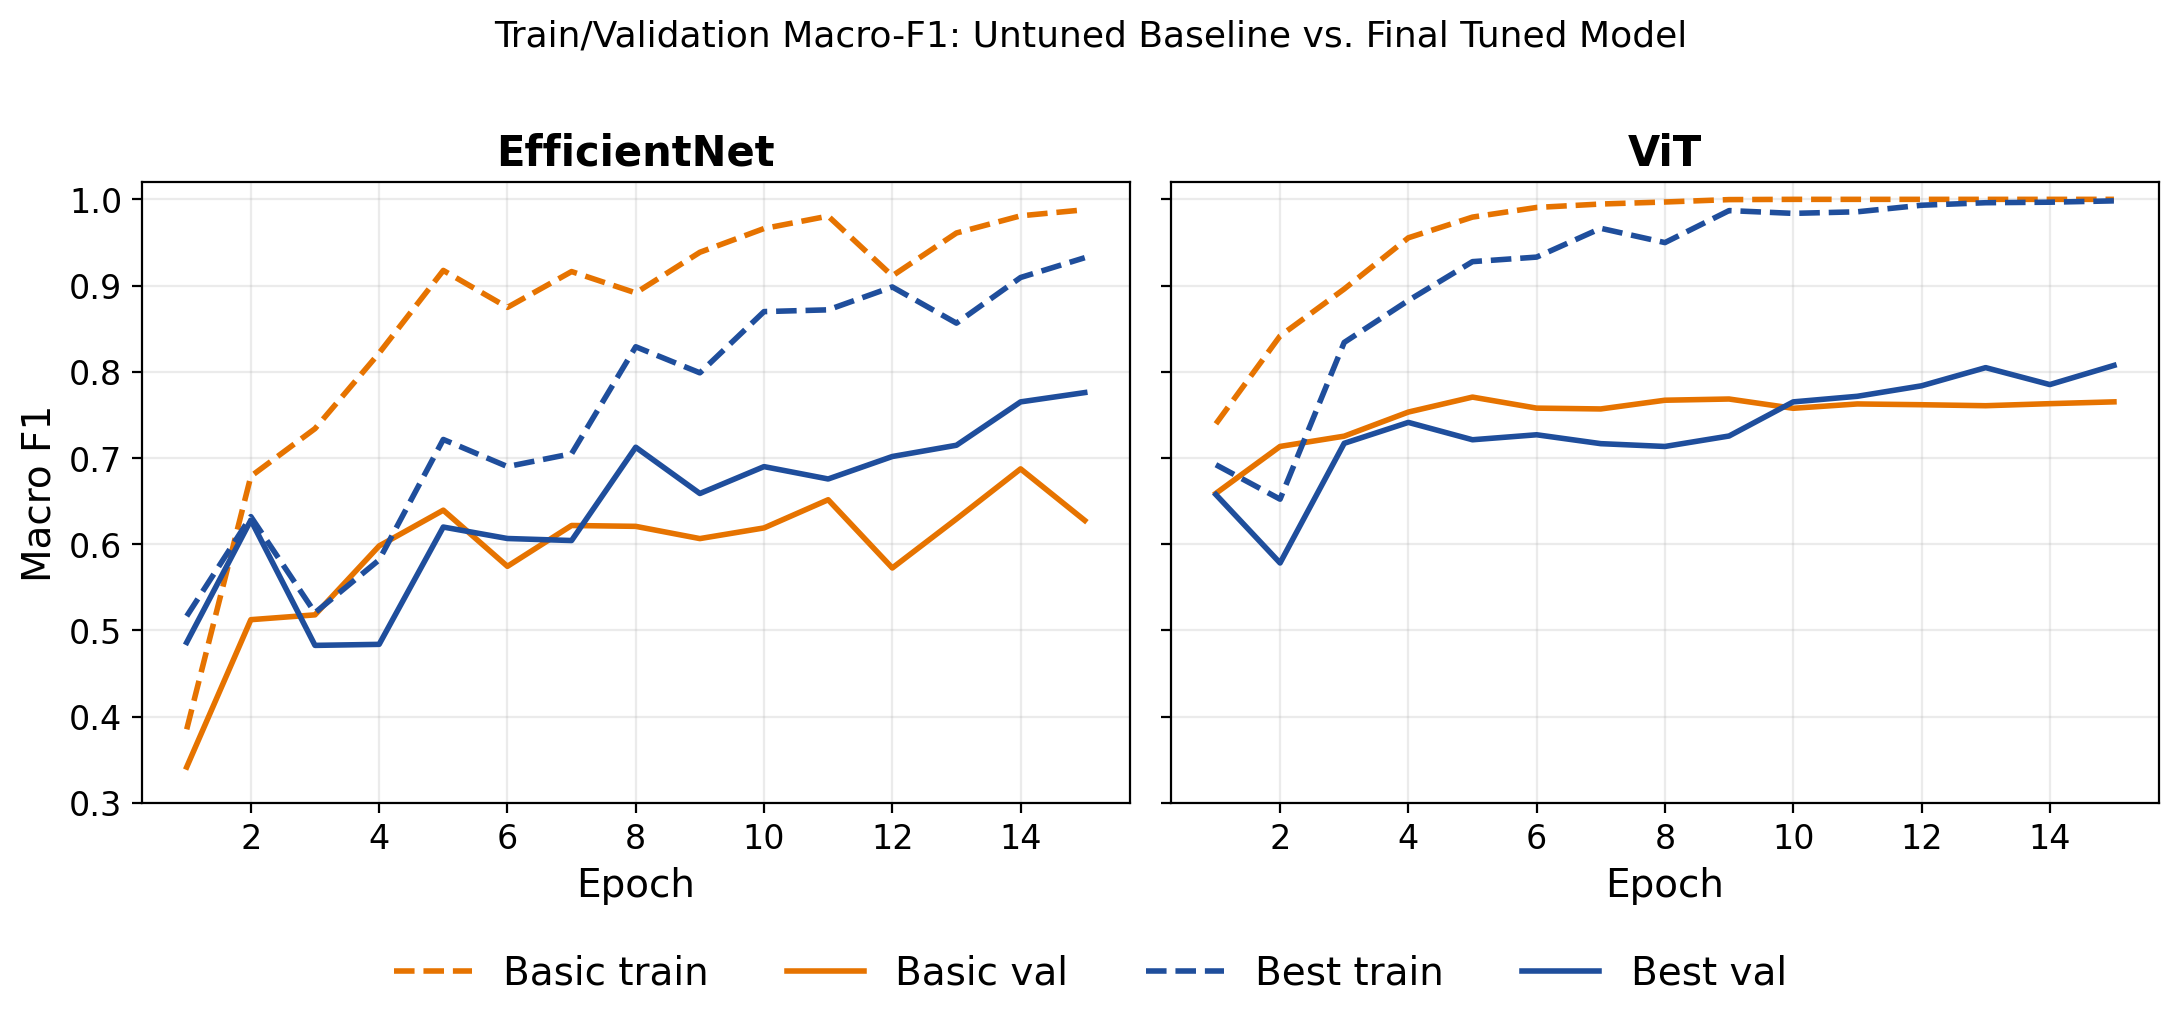
\includegraphics[width=\linewidth]{basic_vs_best_learning_curves.png}
	\caption{Learning curve of baseline and final tuned models for EfficientNet (left) and ViT (right)}
	\label{fig:performance}
\end{figure}


\subsection{Faithfulness}
\label{sec:faithfulness}

Figure~\ref{fig:faithfulness} shows deletion and insertion curves,
macro-averaged predicted-class probability as pixels are removed
(deletion, lower AUC is more faithful) or added back
(insertion, higher AUC is more faithful) in the order each model's heatmap
ranks them, following RISE~\cite{petsiuk2018rise}, against a random-order
baseline for each model. On deletion, EfficientNet's Grad-CAM is markedly more
faithful than chance (AUC 0.174 vs.\ a random-order baseline of 0.538) and
more faithful than ViT's attention rollout in absolute terms (0.646), which is
itself only slightly better than its own random baseline (0.679). On
insertion, the picture is mixed rather than confirmatory: ViT's rollout beats
its random baseline as expected (0.430 vs.\ 0.301), but EfficientNet's
Grad-CAM insertion AUC (0.203) is \emph{below} its own random baseline
(0.291), the opposite of what a faithful ranking should produce. We do not yet
have an explanation for this discrepancy between EfficientNet's strong
deletion result and weak insertion result, and we flag it rather than resolve
it here; one candidate is that Grad-CAM's coarse, blurred localization ranks
pixels correctly at a regional level but not finely enough within a region for
insertion order to matter, though this needs a dedicated check before we treat
it as an explanation rather than a guess.

\begin{figure}[h]
\centering
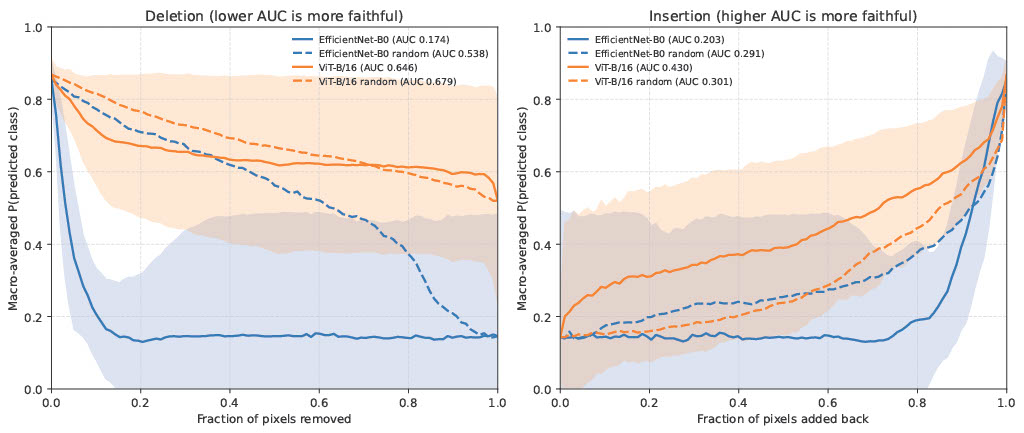
\includegraphics[width=\linewidth]{faithfulness_curves.jpg}
\caption{Deletion (left) and insertion (right) faithfulness curves, macro-averaged predicted-class probability vs.\ fraction of pixels removed/added, for both models against a random-order baseline.}
\label{fig:faithfulness}
\end{figure}

\subsection{Localization}
\label{sec:localization}

Table~\ref{tab:localization} reports IoU and pointing-game hit-rate against
HAM10000's ground-truth lesion segmentation masks, computed with a shared,
architecture-agnostic evaluator (percentile thresholding, top 20\% of heatmap
values) applied unchanged to both Grad-CAM and attention-rollout outputs,
over all 1{,}002 test images (single seed, 42).

\begin{table}[h]
\centering
\footnotesize
\setlength{\tabcolsep}{3pt}
\caption{Localization against ground-truth lesion masks, best checkpoints, $n=1002$, seed 42.}
\label{tab:localization}
\begin{tabular}{lccc}
\toprule
Model & Method & IoU & PG \\
\midrule
EfficientNet-B0 & Grad-CAM & $0.466{\pm}0.177$ & 0.983 \\
ViT-B/16 & Rollout & $0.401{\pm}0.186$ & 0.650 \\
\bottomrule
\end{tabular}
\end{table}

EfficientNet's Grad-CAM localizes more tightly than ViT's rollout on both
metrics. The more informative result, though, is what changed between the
pre-tuning checkpoint (the audited configuration from
Section~\ref{sec:approach}, before the dropout fix) and the final tuned
checkpoint, shown in Table~\ref{tab:localization-delta}.

\begin{table}[h]
\centering
\footnotesize
\setlength{\tabcolsep}{3pt}
\caption{Localization before vs.\ after the fixes in Section~\ref{sec:approach} and the regularization work in Section~\ref{sec:effnet-overfit}.}
\label{tab:localization-delta}
\begin{tabular}{llccc}
\toprule
Model & Metric & Pre & Best & $\Delta$ \\
\midrule
\multirow{2}{*}{EfficientNet-B0} & IoU & $0.484{\pm}0.182$ & $0.466{\pm}0.177$ & $-0.018$ \\
 & PG & 0.973 & 0.983 & $+0.010$ \\
\midrule
\multirow{2}{*}{ViT-B/16} & IoU & $0.300{\pm}0.190$ & $0.401{\pm}0.186$ & $+0.101$ \\
 & PG & 0.454 & 0.650 & $+0.196$ \\
\bottomrule
\end{tabular}
\end{table}

ViT's localization improves substantially with the tuned checkpoint: IoU
rises about a third in relative terms and pointing-game hit-rate rises
nearly 20 points, while EfficientNet's numbers move only within noise. We
read this as an extension of the audit finding in
Section~\ref{sec:approach}: the pre-tuning ViT checkpoint had
\texttt{hidden\_dropout\_prob} and \texttt{attention\_probs\_dropout\_prob}
both at $0.0$, so its attention was less regularized, and its rollout maps
were correspondingly noisier and more diffuse before the fix. The same
configuration bug that inflated ViT's apparent training instability also
degraded the quality of its explanations, not only its accuracy.

\subsection{Summary of results so far}
\label{sec:results-summary}

All three axes are now measured, and two of them agree while one remains
unresolved. Classification favors ViT (Section~\ref{sec:classification}).
Localization favors EfficientNet on both IoU and pointing-game
(Section~\ref{sec:localization}), and deletion faithfulness favors
EfficientNet by a wide margin (Section~\ref{sec:faithfulness}), so two of our
three explanation-quality signals converge on EfficientNet's Grad-CAM being
the more trustworthy explanation. The exception is EfficientNet's insertion
AUC, which remains below its own random baseline
(Section~\ref{sec:faithfulness}) and is still unexplained; we do not let this
override the converging deletion and localization evidence, but we also do
not consider it resolved.

\section{Discussion}
\label{sec:discussion}

\subsection{Problem Structure and Architectural Alignment}

Skin lesion classification is a \emph{bounded localization task}: diagnosis
depends on fine-grained texture and morphology \emph{within} the lesion, with
robustness to background artifacts. This aligns naturally with EfficientNet's
local-to-global hierarchy and less obviously with ViT's global-first
attention. Our results read as evidence for both perspectives: EfficientNet's
Grad-CAM is more faithful on deletion and localizes more tightly on both IoU
and pointing-game hit-rate (Sections~\ref{sec:faithfulness}--\ref{sec:localization}),
consistent with locality-biased features tracking diagnostic texture
directly, while ViT reaches higher test accuracy
(Section~\ref{sec:classification}), consistent with global context, e.g.\
lesion asymmetry across the full extent of a lesion, adding information a
purely local model cannot see. We hold this reading loosely: EfficientNet's
insertion AUC contradicts its own deletion result
(Section~\ref{sec:faithfulness}), and the checkpoint mismatch noted in
Section~\ref{sec:results-summary} means faithfulness and localization are not
yet measured on identical checkpoints, so we are not calling this fully
settled, even though two of three explanation-quality axes now point the same
direction.

\subsection{Model Components: Learned and Fixed}

\textbf{Learned:} the 7-way classification head (trained from scratch) and
the backbone (unfrozen and fine-tuned in Stage 2). \textbf{Fixed:} Grad-CAM
and attention rollout, both post-hoc and parameter-free, plus softmax
normalization and argmax classification. This split is also empirically
supported: unfreezing the backbone already in Stage 1, then retuning its
learning rate per variant, never exceeded the frozen-Stage-1 baseline's
validation macro-F1 (0.8074) by more than epoch-to-epoch noise, so a frozen
Stage 1 is at least as good and cheaper to tune.

\subsection{Input/Output Representations}

Both networks take $224\times224$ RGB input normalized with ImageNet channel
statistics, to stay aligned with each pretrained backbone. Output logits pass
through softmax to probabilities, with the predicted class $\arg\max_i p_i$;
the faithfulness tests (Section~\ref{sec:faithfulness}) track
$p(\text{predicted class})$ directly, not the logits or heatmap.

\subsection{Loss Function and Regularization}

Class-weighted cross-entropy addresses the label imbalance (melanocytic
nevus 67\%, dermatofibroma 1\%). Regularization behaved less predictably.
Dropout alone left EfficientNet's validation macro-F1 essentially flat
across a $0.2$--$0.5$ sweep (Section~\ref{sec:effnet-overfit}), which
follows from where EfficientNet-B0 places its only dropout layer:
immediately before the final linear layer, never touching the MBConv blocks
that make up most of the unfrozen backbone. \texttt{drop\_connect\_rate} and
weight decay each closed only a small part of the gap alone; augmentation,
combined with moderate dropout and drop-connect rate, meaningfully narrowed
it. ViT shows the opposite sensitivity: dropout $0.2$ is its best single
setting, while the same augmentation that helped EfficientNet reduces ViT's
validation macro-F1 at every dropout level tested. We read this not as ViT
having ``inherent attention-based regularization'' but as having less
inductive bias to fall back on, so perturbing input geometry interferes with
learning positional structure rather than adding beneficial invariance as it
does for a convolutional model.

\subsection{Transfer Learning and Implementation}

Starting from ImageNet-pretrained weights was necessary at this scale: both
models converge within 20 epochs total (5 Stage-1 plus 15 Stage-2) on
7{,}470 unique lesions, far fewer epochs and data than random initialization
would need, protected by the two-stage schedule (Section~\ref{sec:approach}).
Both models are implemented in PyTorch with Hugging Face
\texttt{transformers}, our own Grad-CAM~\cite{selvaraju2017gradcam} and
attention-rollout~\cite{abnar2020attention} implementations, and RISE-style
~\cite{petsiuk2018rise} faithfulness metrics; code and checkpoints are public
(footnote, Section~\ref{sec:approach}).

\section{Conclusion}
\label{sec:conclusion}

This study compared a convolutional network and a vision transformer for
explainable skin lesion classification on HAM10000, across three axes:
classification accuracy, faithfulness, and localization. ViT-B/16 reaches
higher test macro-F1 than EfficientNet-B0 (0.773 vs.\ 0.696) and generalizes
with a narrower validation-test gap (Section~\ref{sec:classification}). On
the two explanation-quality axes, EfficientNet's Grad-CAM converges on being
the more trustworthy explanation: it is markedly more faithful on deletion
and localizes more tightly against ground-truth lesion masks on both IoU and
pointing-game hit-rate (Sections~\ref{sec:faithfulness}--\ref{sec:localization}).
This is not a unanimous verdict: EfficientNet's insertion AUC falls below its
own random baseline, a result we flag but have not explained, so we stop
short of calling faithfulness fully settled even though localization now
corroborates the deletion result. Taken together, the results point toward
the trade-off the Introduction set out to test: the architecture whose
local, convolutional structure produces more trustworthy explanations is not
the architecture that classifies most accurately.

A second, independent finding came out of our hyperparameter work: the two
architectures overfit for different reasons and respond to different
regularization fixes (Section~\ref{sec:effnet-overfit}), and the same
code-audit-driven fix to ViT's zero-dropout configuration
(Section~\ref{sec:approach}) that helped classification also substantially
improved ViT's localization quality (IoU $+0.101$, pointing-game $+0.196$,
Section~\ref{sec:localization}) while leaving EfficientNet's localization
essentially unchanged. This links a fine-tuning configuration bug directly to
explanation quality, not just accuracy: regularization choices should be
audited for their effect on interpretability, not only on validation
accuracy.

\section{Future Work}
\label{sec:future-work}
Three items are immediate and finish the study as scoped rather than extend
it. First, the faithfulness curves in Figure~\ref{fig:faithfulness} predate
the regularization fixes in Section~\ref{sec:effnet-overfit} and should be
regenerated on the same tuned checkpoints used for localization
(Section~\ref{sec:localization}), so all three axes are measured
consistently. Second, both results reported here are single-seed (seed 42);
the Evaluation Plan calls for a 3-seed mean$\pm$std across the full protocol
and a qualitative 10-correct/10-misclassified overlay comparison, both still
outstanding. Third, EfficientNet's insertion AUC falling below its random
baseline is unexplained; before treating the deletion result as evidence of
faithful explanations, this needs a direct check, e.g.\ whether Grad-CAM's
coarse spatial resolution ranks pixels correctly at a regional level but not
finely enough for insertion order to matter.

Beyond finishing the current comparison, three extensions would strengthen
it: evaluating on a second dataset (e.g.\ ISIC 2018, already supported by our
download script) to test whether the architecture-specific overfitting
pattern (Section~\ref{sec:effnet-overfit}) is a property of these
architectures or an artifact of HAM10000's size; a joint objective optimizing
for faithfulness alongside accuracy, rather than measuring it only post hoc,
to test whether the accuracy-faithfulness trade-off we observe is fundamental
or an artifact of training for accuracy alone; and a human study, since our
metrics only proxy clinical trust rather than measuring whether a better
heatmap changes a clinician's confidence or diagnostic accuracy.

\textbf{Broader impact:} the architecture-specific overfitting pattern
(Section~\ref{sec:effnet-overfit}) follows from where each architecture
places its regularization, not from anything skin-specific, so we expect it
and our faithfulness/localization methodology to generalize to other small
medical imaging datasets; HAM10000's skew toward European-institution data
remains a limitation for any clinical
deployment.

% ============================================================================
% TEAM CONTRIBUTIONS (does not count toward page limit)
% ============================================================================
\section*{Team Contributions}


\begin{table*}[t]
\begin{center}
\begin{tabular}{|p{3cm}|p{5cm}|p{8cm}|}
\hline
Team Member & Contributed Aspects & Details \\
\hline\hline
Xiaoyan Xing & Project Proposal, Implementation, Hyperparameter Tuning, Fine Tuning, Analysis & Review and edited project proposal. Implemented ViT Attention rollout framework and heatmap generation. Hyperparameter tuning and for both EfficientNet and ViTEfficientNet's overfitting mechanism (dropout $\rightarrow$ drop-connect rate $\rightarrow$ weight decay $\rightarrow$ augmentation ablations, Section 3.2); ViT dropout and weighted-vs-unweighted cross-entropy ablations; final trained checkpoints. \\
\hline
Sebastian Gonzalez & Project Coordination, Project Proposal, Implementation, Fine-Tuning, Analysis & Created Github and HuggingFace repositories. Reviewed and edited project proposal. Implemented Two-stage fine-tuning pipeline and repository (device auto-detection, checkpoint publishing). Implemented faithfulness (deletion/insertion) evaluation code, Section 3.3. \\
\hline
Somayeh Bahrami & Project Proposal, Implementation, Analysis,Report writing & Review and edited project proposal. Localization evaluation, IoU and pointing-game scoring against HAM10000 segmentation masks, Section 3.4.\\
\hline
Ka Wing Ariel Lee & Project Coordination, Project Proposal, Implementation, Fine-Tuning, Analysis & Coordinated communication. Set up shared documentation and infrastructure for the team. Drafted project proposal. Implemented EfficientNet Grad-CAM framework and heatmap generation. Reviewed and revised the two-stage fine-tuning protocol. Reviewed and edited report.\\
\hline
\end{tabular}
\end{center}
\caption{Contributions of team members.}
\label{tab:contributions}
\end{table*}


% ============================================================================
% REFERENCES (does not count toward page limit)
% ============================================================================

\begin{thebibliography}{99}

\bibitem{esteva2017dermatologist}
Esteva, A., Kuprel, B., Novoa, R. A., Ko, J., Swetter, S. M., Blau, H. M., \& Thrun, S. (2017).
``Dermatologist-level classification of skin cancer with deep neural networks.''
\textit{Nature}, 542(7639), 115--118.

\bibitem{tschandl2018ham10000}
Tschandl, P., Rosendahl, C., \& Kittler, H. (2018).
``The HAM10000 dataset, a large collection of multi-source dermatoscopic images of common pigmented skin lesions.''
\textit{Scientific Data}, 5, 180161.

\bibitem{tan2019efficientnet}
Tan, M., \& Le, Q. (2019).
``EfficientNet: Rethinking model scaling for convolutional neural networks.''
\textit{ICML}.

\bibitem{dosovitskiy2021vit}
Dosovitskiy, A., Beyer, L., Kolesnikov, A., Weissenborn, D., Zhai, X., Unterthiner, T., Dehghani, M., Minderer, M., Heigold, G., Gelly, S., Uszkoreit, J., \& Houlsby, N. (2021).
``An image is worth 16x16 words: Transformers for image recognition at scale.''
\textit{ICLR}.

\bibitem{kuntal2025bridging}
Kuntal, Y. A., \& Bhat, A. (2025).
``Bridging CNNs and transformers for skin cancer detection: A comparative analysis.''
\textit{2025 7th International Conference on Information Systems and Computer Networks (ISCON)}.

\bibitem{selvaraju2017gradcam}
Selvaraju, R. R., Cogswell, M., Das, A., Vedantam, R., Parikh, D., \& Batra, D. (2017).
``Grad-CAM: Visual explanations from deep networks via gradient-based localization.''
\textit{ICCV}.

\bibitem{abnar2020attention}
Abnar, S., \& Zuidema, W. (2020).
``Quantifying attention flow in transformers.''
\textit{ACL}.

\bibitem{kozachok2026melanoscope}
Kozachok, E. S., \& Seregin, S. S. (2026).
``Clinical validation of the Melanoscope AI mobile dermoscopy clinical decision support system.''
\textit{arXiv preprint arXiv:2605.27561}.

\bibitem{petsiuk2018rise}
Petsiuk, V., Das, A., \& Saenko, K. (2018).
``RISE: Randomized input sampling for explanation of black-box models.''
\textit{BMVC}.

\bibitem{samek2017evaluating}
Samek, W., Binder, A., Montavon, G., Lapuschkin, S., \& M\"uller, K.-R. (2017).
``Evaluating the visualization of what a deep neural network has learned.''
\textit{IEEE Transactions on Neural Networks and Learning Systems}, 28(11), 2660--2673.

\bibitem{gebru2021datasheets}
Gebru, T., Morgenstern, J., Vecchione, B., Vaughan, J. W., Wallach, H., Daum\'e III, H., \& Crawford, K. (2021).
``Datasheets for datasets.''
\textit{Communications of the ACM}, 64(12), 86--92.

\bibitem{kumar2022finetuning}
Kumar, A., Raghunathan, A., Jones, R., Ma, T., \& Liang, P. (2022).
``Fine-tuning can distort pretrained features and underperform out-of-distribution.''
\textit{ICLR}.

\bibitem{howard2018ulmfit}
Howard, J., \& Ruder, S. (2018).
``Universal language model fine-tuning for text classification.''
\textit{ACL}.

\bibitem{tomihari2024ntk}
Tomihari, A., \& Sato, I. (2024).
``Understanding linear probing then fine-tuning language models from NTK perspective.''
\textit{NeurIPS}.

\bibitem{lee2023surgical}
Lee, Y., Chen, A. S., Tajwar, F., Kumar, A., Yao, H., Liang, P., \& Finn, C. (2023).
``Surgical fine-tuning improves adaptation to distribution shifts.''
\textit{ICLR}.

\bibitem{davila2024comparison}
Davila, A., Colan, J., \& Hasegawa, Y. (2024).
``Comparison of fine-tuning strategies for transfer learning in medical image classification.''
\textit{Image and Vision Computing}, 146, 105012.

\bibitem{loshchilov2019adamw}
Loshchilov, I., \& Hutter, F. (2019).
``Decoupled weight decay regularization.''
\textit{ICLR}.

\end{thebibliography}

\appendix
\section{Appendix}

\subsection{Full Fine-Tuning Strategy Depth Sweep}
\label{app:strategy-full}

Table~\ref{tab:strategy-comparison-full} gives the complete depth sweep
behind the summary in Table~\ref{tab:strategy-comparison}
(Section~\ref{sec:strategy}).

\begin{table*}[t]
	\centering

	{\fontsize{10}{11}\selectfont
		\renewcommand{\arraystretch}{0.9}
		\setlength{\extrarowheight}{0pt}
		\setlength{\tabcolsep}{3pt}

		\begin{tabular}{@{}p{0.54\textwidth}@{\hspace{0.02\textwidth}}p{0.44\textwidth}@{}}

			% Super row
			\multicolumn{1}{c}{\tablestrut\textbf{Strategy 1}} &
			\multicolumn{1}{c}{\tablestrut\textbf{Strategy 2}} \\
			\hline

			% Top-left subtable
			\begin{tabularx}{\linewidth}
				{@{}>{\centering\arraybackslash}p{0.24\linewidth}
					*{4}{>{\centering\arraybackslash}X}@{}}

				\tablestrut Unfreeze Layer & 2 & 4 & 6 & all \\
				\hline
				\multicolumn{5}{c}{\tablestrut\textbf{EfficientNet}} \\
				\hline
				\tablestrut Train-mF1 & 0.8540 & 0.9341 & 0.9571 & 0.9880 \\
				\hline
				\tablestrut Val-mF1 & 0.5631 & 0.5998 & 0.6131 & 0.6874 \\

			\end{tabularx}

			&

			% Top-right subtable
			\begin{tabularx}{\linewidth}
				{@{}>{\centering\arraybackslash}p{0.30\linewidth}
					*{3}{>{\centering\arraybackslash}X}@{}}

				\tablestrut Unfreeze Layer & 2 & 4 & 6 \\
				\hline
				\multicolumn{4}{c}{\tablestrut\textbf{EfficientNet}} \\
				\hline
				\tablestrut Train-mF1 & 0.9943 & 0.9919 & 0.9986 \\
				\hline
				\tablestrut Val-mF1 & 0.6496 & 0.6488 & 0.6866 \\

			\end{tabularx}

			\\
			\hline

			% Bottom-left subtable
			\begin{tabularx}{\linewidth}
				{@{}>{\centering\arraybackslash}p{0.24\linewidth}
					*{4}{>{\centering\arraybackslash}X}@{}}

				\multicolumn{5}{c}{\tablestrut\textbf{ViT}} \\
				\hline
				\tablestrut Train-mF1 & 0.8960 & 0.9802 & 0.9984 & 1 \\
				\hline
				\tablestrut Val-mF1 & 0.6956 & 0.7211 & 0.7477 & 0.7707 \\

			\end{tabularx}

			&

			% Bottom-right subtable
			\begin{tabularx}{\linewidth}
				{@{}>{\centering\arraybackslash}p{0.30\linewidth}
					*{3}{>{\centering\arraybackslash}X}@{}}

				\multicolumn{4}{c}{\tablestrut\textbf{ViT}} \\
				\hline
				\tablestrut Train-mF1 & 1 & 1 & 1 \\
				\hline
				\tablestrut Val-mF1 & 0.7501 & 0.7437 & 0.7577 \\

			\end{tabularx}

			\\
			\hline

		\end{tabular}
	}

	\caption{Strategy 1 vs. Strategy 2 full depth sweep, training and validation MacroF1 (untuned hyperparameters).}
	\label{tab:strategy-comparison-full}

\end{table*}

\subsection{Full Hyperparameter Search Grid}
\label{app:hp-grid}

Full grid swept jointly for each architecture in
Section~\ref{sec:model-selection}:

\noindent\textbullet\ dropout: \{0.1, 0.2, 0.3, 0.4\}\\
\textbullet\ drop\_connect\_rate: \{0.1, 0.2, 0.3, 0.4\}\\
\textbullet\ augmentation: \{True, False\}\\
\textbullet\ Phase 1 lr: \{$1e^{-4}$, $4e^{-4}$, $8e^{-4}$, $1e^{-3}$, $5e^{-3}$, $8e^{-3}$, $1e^{-2}$\}\\
\textbullet\ Phase 2 lr: \{$1e^{-5}$, $2e^{-5}$, $4e^{-5}$, $8e^{-5}$, $1e^{-4}$, $5e^{-4}$,  $8e^{-4}$\}\\
\textbullet\ weight decay: \{0.01, 0.05, 0.1, 0.2\}\\
\textbullet\ batch size: \{8, 16, 32\}\\
\textbullet\ warmup\_ratio: \{0.1, 0.2\}

\subsection{Full Weighted vs. Unweighted Loss Comparison}
\label{app:weighted-unweighted-full}

Table~\ref{tab:weighted-unweighted-full} gives the full validation/test
breakdown behind the summary in Table~\ref{tab:weighted-unweighted}
(Section~\ref{sec:model-selection}).

\begin{table*}
	\centering

	{\fontsize{10}{11}\selectfont
		\renewcommand{\arraystretch}{0.9}
		\setlength{\extrarowheight}{0pt}
		\setlength{\tabcolsep}{3pt}

		\begin{tabularx}{\textwidth}
			{@{}>{\centering\arraybackslash}p{0.16\textwidth}
				*{8}{>{\centering\arraybackslash}X}@{}}

			% Shared meta row: 9 columns total
			\tablestrut\textbf{ } &
			Avg\_tr\_mF1 &
			Avg\_v\_mF1 &
			Gap &
			Best\_tr\_mF1 &
			Best\_v\_mF1 &
			Best\_v\_acc &
			Test\_mF1 &
			Test\_acc \\
			\hline

			% EfficientNet subtable
			\multicolumn{9}{c}
			{\tablestrut\textbf{EfficientNet}} \\
			\hline

			\tablestrut{Weighted} &
			0.6394 &
			0.5601 &
			0.0793 &
			0.9323 &
			0.7759 &
			0.7964 &
			0.6546 &
			0.7036 \\
			\hline

			\tablestrut{Unweighted} &
			0.7010 &
			0.5956 &
			0.1054 &
			0.9853 &
			0.7378 &
			0.7428 &
			0.6405 &
			0.6559 \\
			\hline\hline

			% ViT subtable
			\multicolumn{9}{c}
			{\tablestrut\textbf{ViT}} \\
			\hline

			\tablestrut{Weighted} &
			0.7176 &
			0.6069 &
			0.1107 &
			0.9982 &
			0.8074 &
			0.7893 &
			0.7478 &
			0.7511 \\
			\hline

			\tablestrut{Unweighted} &
			0.7495 &
			0.6145 &
			0.1350 &
			0.9999 &
			0.7835 &
			0.7684 &
			0.7159 &
			0.7013 \\
			\hline

		\end{tabularx}
	}

	\caption{Weighted vs. unweighted loss function comparison, full breakdown. Best\_tr\_mF1/Best\_v\_mF1/Best\_v\_acc are reported at the epoch of peak validation Macro-F1 (the checkpointed epoch); test metrics are from that checkpoint.}
	\label{tab:weighted-unweighted-full}

\end{table*}

\subsection{Model Architectures}

\begin{figure}[h]
\centering
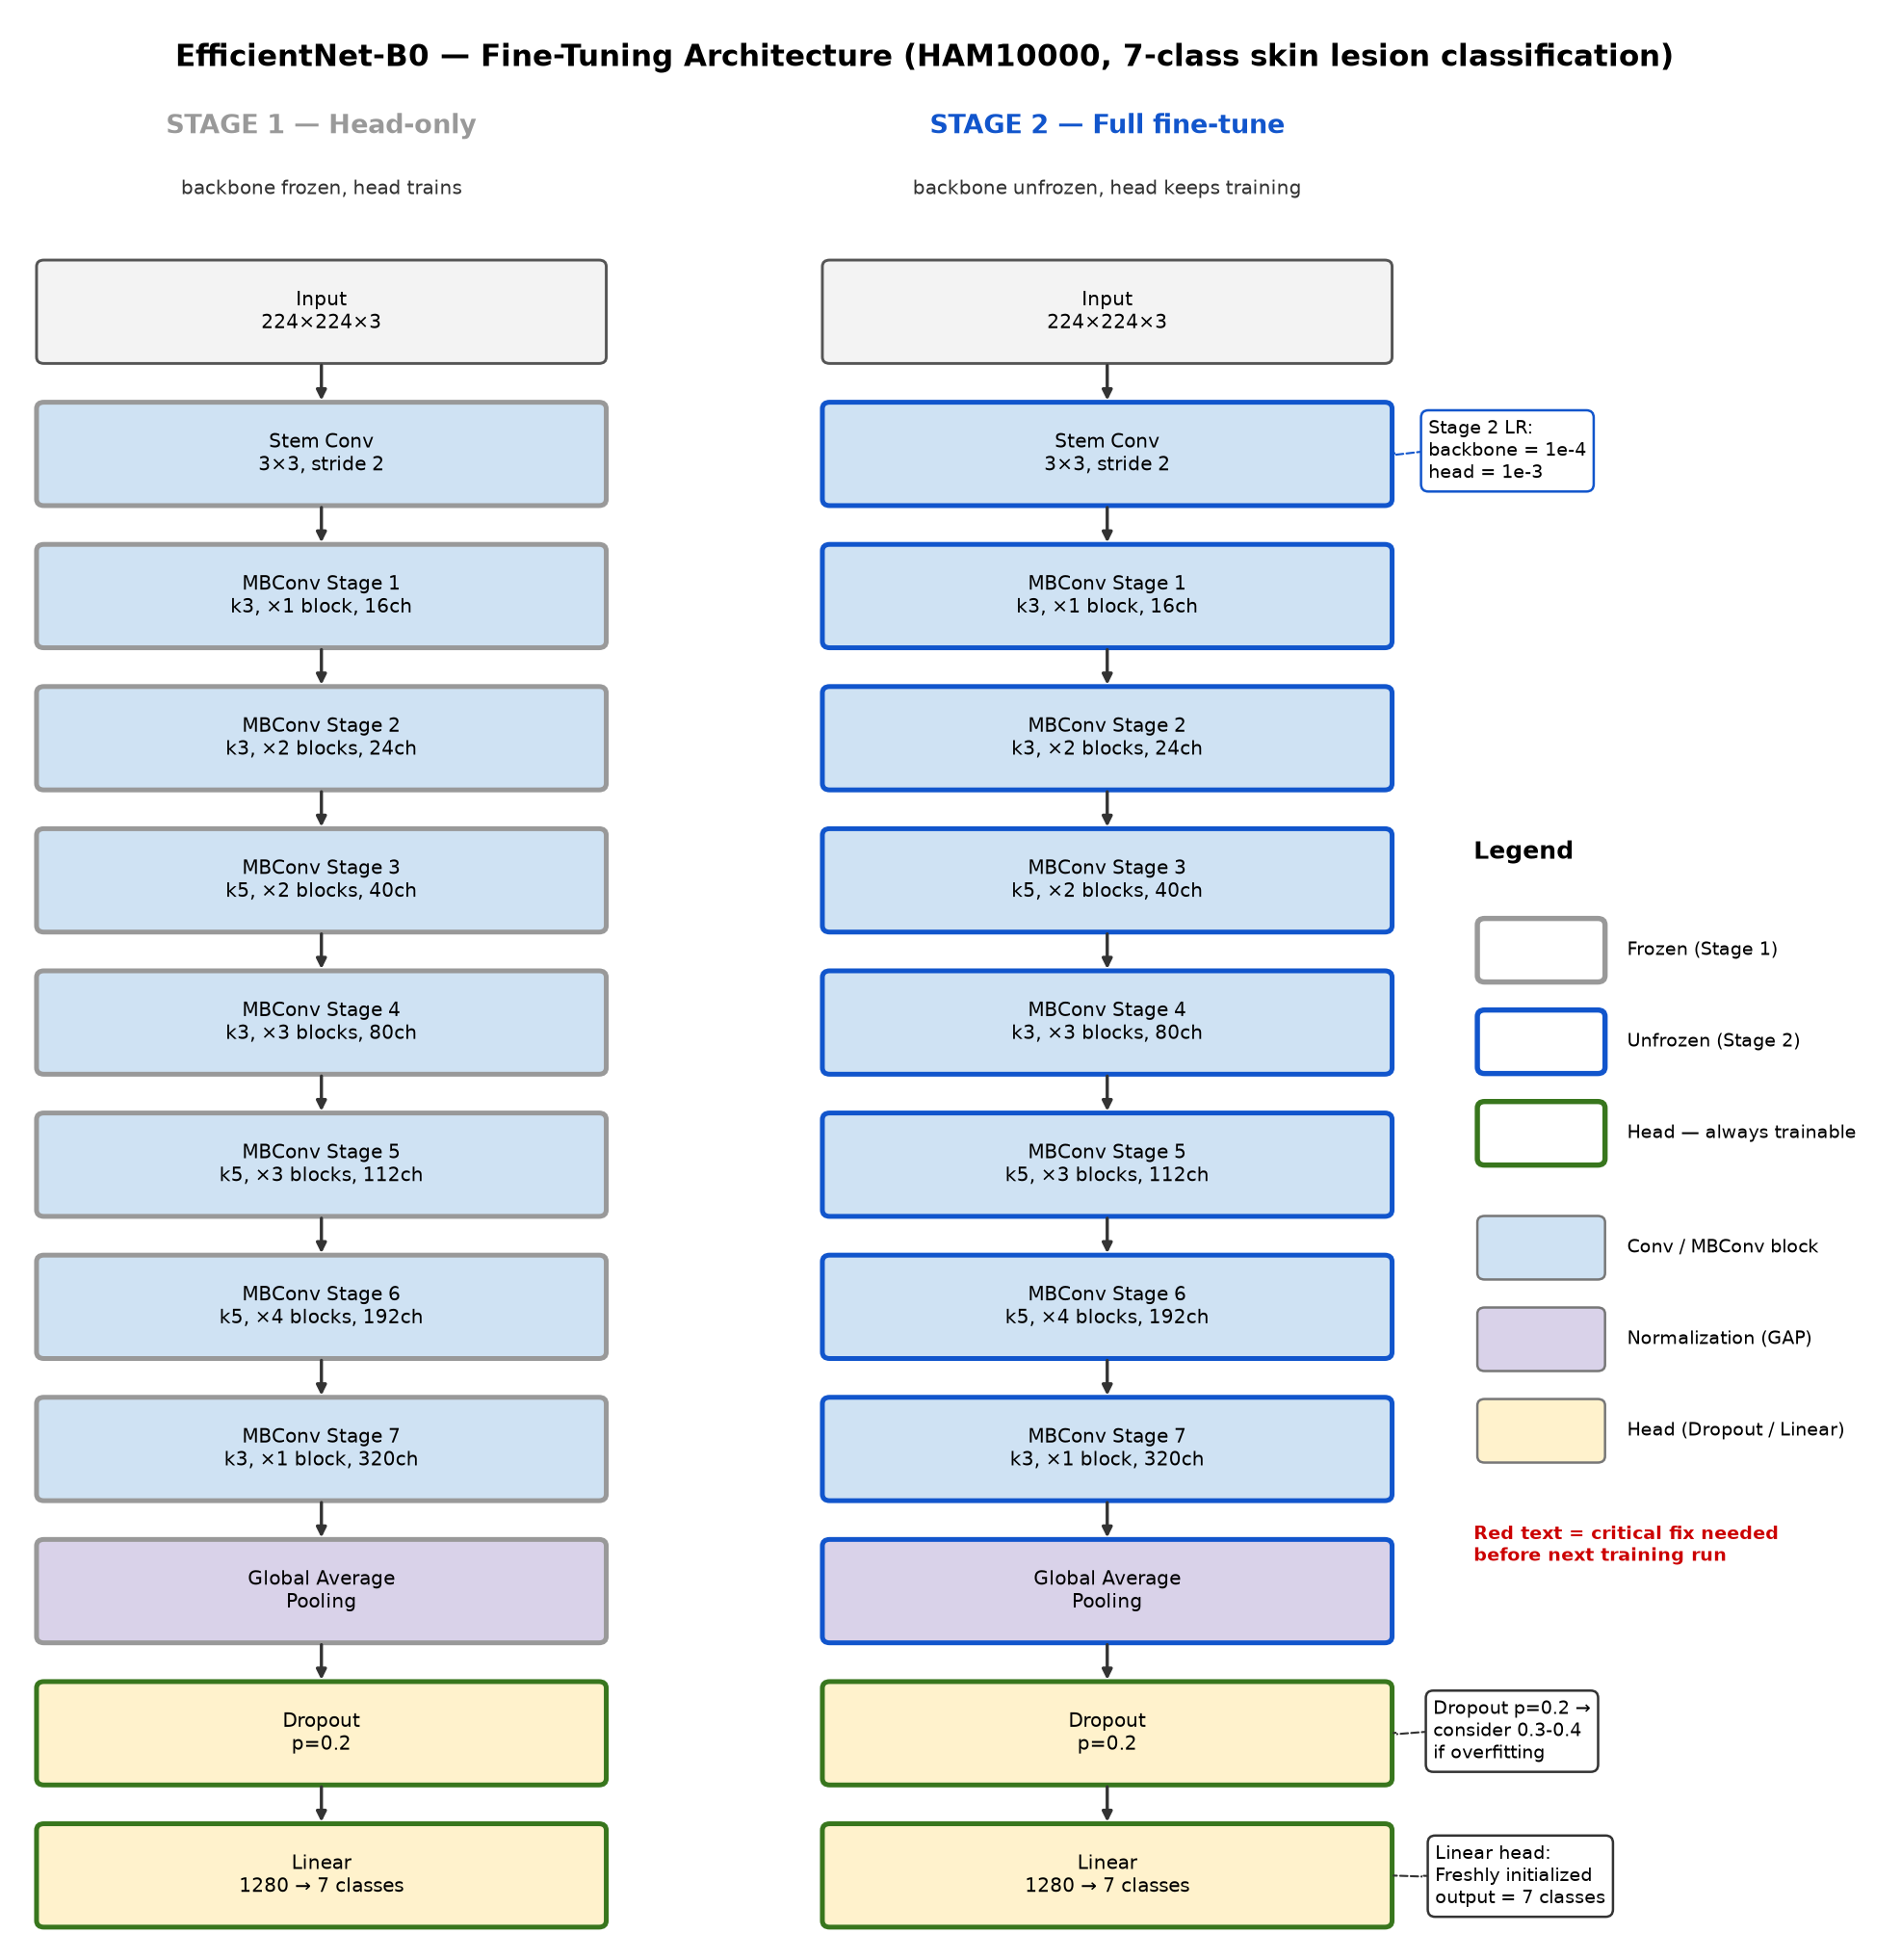
\includegraphics[width=\linewidth]{efficientnet_b0_finetuning_edited.png}
\caption{EfficientNet architecture.}
\label{fig:efficientnet_b0_finetuning_edited}
\end{figure}


\begin{figure}[h]
\centering
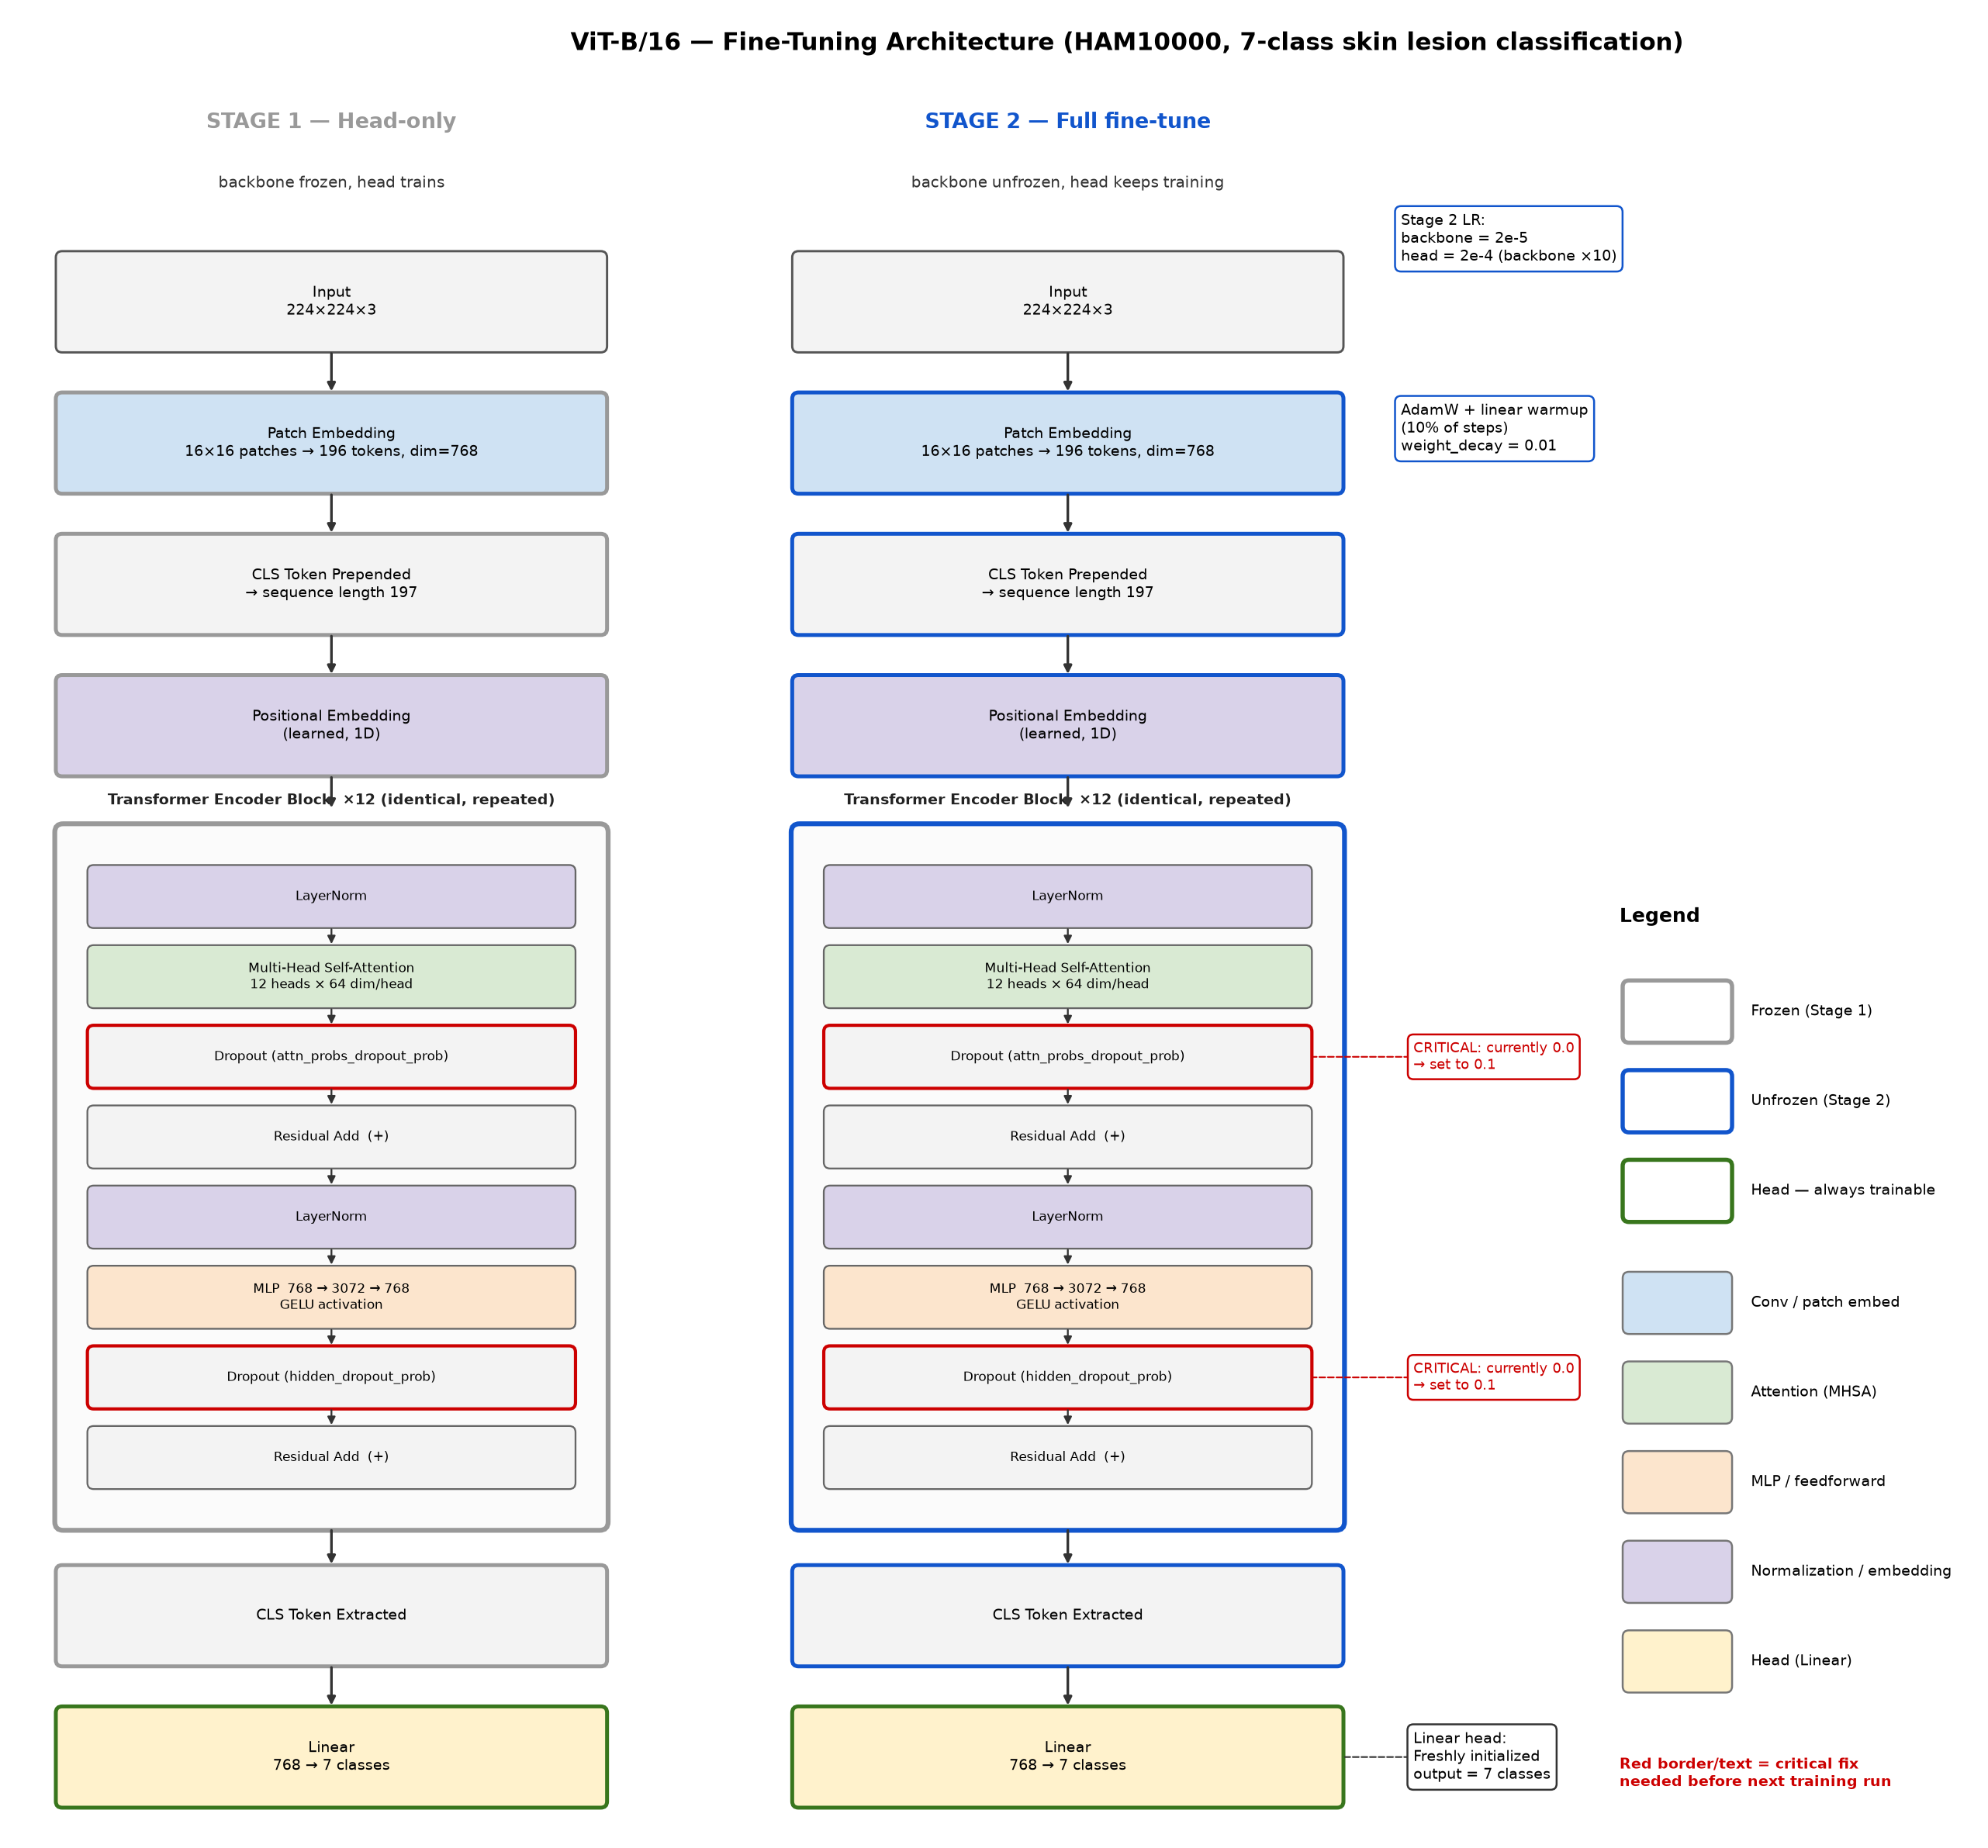
\includegraphics[width=\linewidth]{vit_b16_finetuning_edited.png}
\caption{ViT-B/16 architecture.}
\label{fig:vit_b16_finetuning_edited}
\end{figure}

\end{document}